%!TEX root = ../thesis.tex

\begin{savequote}[75mm]
$\blacktriangleleft$ I faced the challenge of observing molecules with the help of state-of-the-art experimental techniques. Here, the reader must perform one last experiment using, by far, the most advanced observation instrument that we have: the human eye.

\vspace{3pt}

(Hint: watch it horizontally)
\end{savequote}


\chapter{Introduction}\label{chap:introduction}


\vspace{30pt}


\section{Water: a structured material}


Despite being the most familiar and abundant compound on earth, water has captivated humankind for centuries. Since ancient times, for example, humans have wondered at the property of ice to float on liquid water, which is the consequence of water having a lower density as a solid than as a liquid. This anomalous behavior finds its origin in the nature of water to form structures: crystal-like networks that increase the volume of the system when it freezes. This example belongs to a long list of anomalies as compared to other liquids,\!\cite{Russo2018} many of which are linked to the structured character of water. However, in spite of considerable efforts, a precise description of its structural properties remains elusive to date.\!\cite{Ball2008}




In liquid water, hydrogen bonds are considered the intermolecular ``glue'' that gives rise to the structure called the hydrogen-bond network. In this network, each hydrogen bond results from the (mainly electrostatic) bonding between one of the partially positive hydrogen atoms and one of the lone-pair electrons in neighboring water molecules. Thus, each water molecule has the potential to participate in the formation of four hydrogen bonds: donating two (two hydrogen atoms) and accepting two (two lone-pair electrons), as depicted in Figure \ref{MoleculeHStructure}. As was validated in 1933 using X-rays, the perfect arrangement of water molecules leads to a periodic tetrahedral structure.\!\cite{Bernal1933}



Recent studies show, however, that liquid water possesses on average 3.5 hydrogen bonds per molecule in ambient conditions.\!\cite{Soper2000,Wernet2004,Kumar2007} This means that the hydrogen-bond network is defective to the extent that it allows changes in the local coordinates as well as structural rearrangements, which have been observed to occur on a sub-picosecond ($\leq$$10^{-12}$~s) time scale.\!\cite{Lawrence2003,Eaves2005,Fecko2005,Laage2006} As such, the hydrogen-bond network of water is a highly active and adaptive environment. It is thus not surprising that many chemical and biological processes occur in aqueous environments---an excellent environment for life to prosper in.\!\cite{Ball2008c,Bellissent-Funel2016,Ball2017}


\begin{figure}[t!]
	\centering
	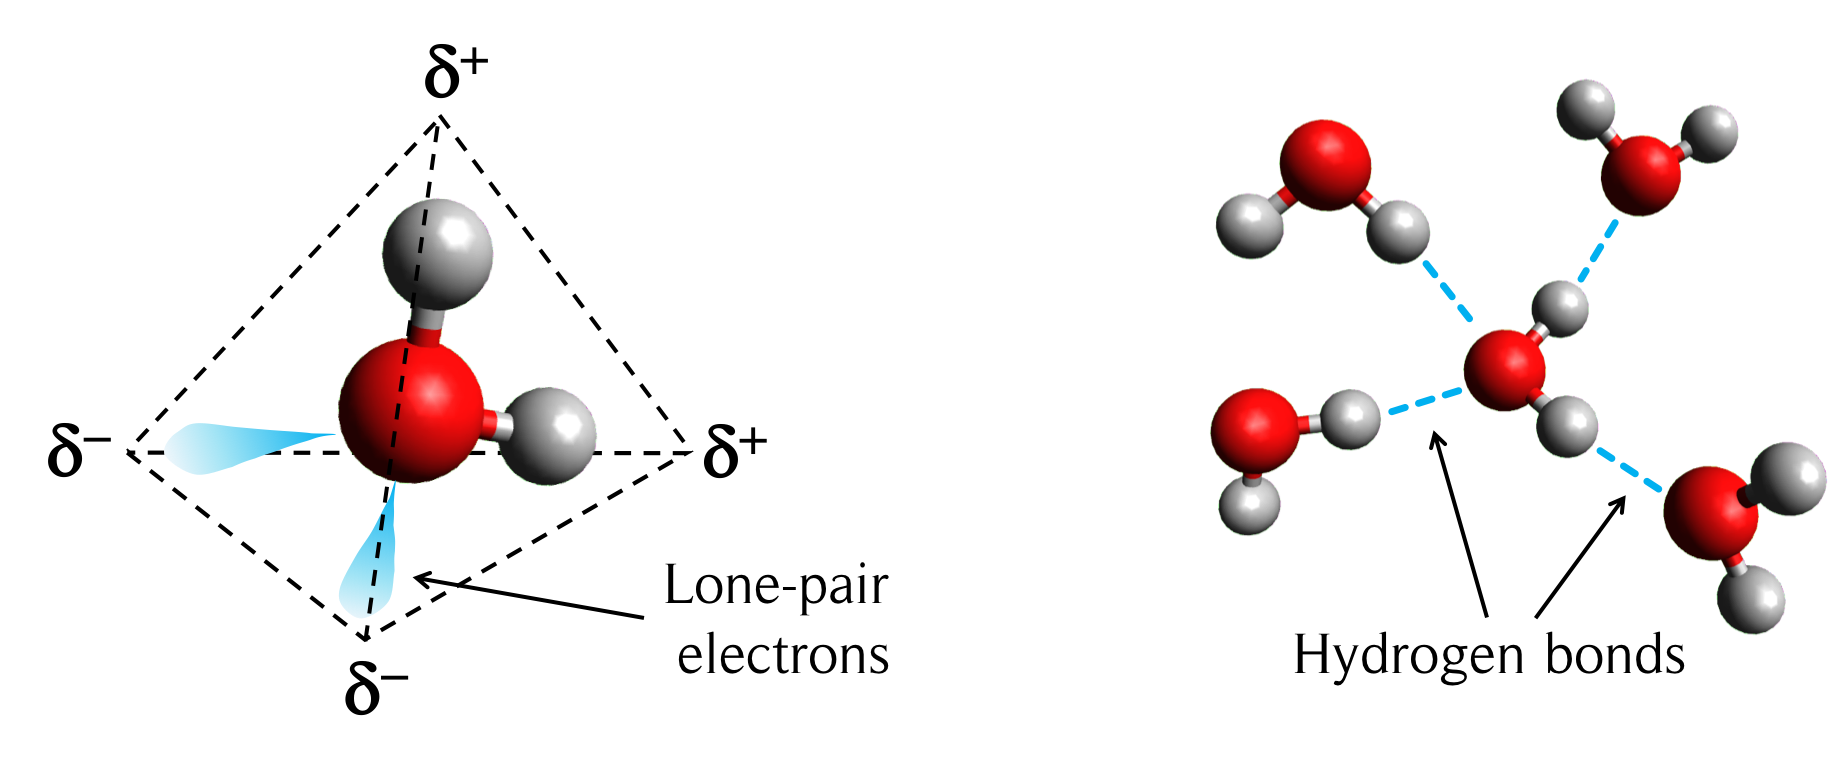
\includegraphics[width=0.8\figwidth]{chapters/Chapter1_Introduction/Graphs/HydrogenBondsC.png} %The local modes are calculated on the XXX level, and reproduced with permission from ref. XXX. 
	\caption{\textbf{Left:} Tetrahedral configuration of a water molecule. \textbf{Right:} Local hydrogen-bond structure of a water molecule that extends to form the so-called hydrogen-bond network of liquid water. }
	\label{MoleculeHStructure}
\end{figure}



Yet, water is often regarded as a stiff liquid, a concept introduced by Marcus,\!\cite{Marcus2009,Marcus2010} in which the hydrogen bonding leads to cooperative dynamics. This cooperativity constrains the mobility of water molecules themselves, as well as the dynamics of other molecules dissolved in water. In aqueous solutions, the solutes can reciprocally affect the cooperative behavior due to discontinuities and defects in the hydrogen-bond network of water. If the concentration of solutes in water is high enough, one can observe changes in the macroscopic properties of water: the viscosity and surface tension increases or decreases depending on the nature of the solute.



\section{The influence of ions on the structure of water}



The way in which ions, among other solutes, modify the structural dynamics of water has been a long-standing question and is an active field of experimental and theoretical research. An accurate description of ion-water interactions is of importance for the study of many chemical and biological processes, ranging from the conformation of proteins to the selection rules for ion exchange in living cells.



In electrolyte solutions, ions generate strong local electric fields that modify the hydrogen-bond structure and induce local molecular ordering in the form of solvation shells. Based on the degree of water structuring in solvation shells, ions are classified as structure makers or structure breakers, concepts coined by Gurney in the 50s.\!\cite{Gurney1953} In this context, while small ions with high surface charge densities are structure makers that form tight solvation shells, large ions form labile solvation structures due to their low surface charge density. 


Most of the work that has been carried out to study ion-water interactions has been reviewed by Yizhak Marcus\!\cite{Marcus1988,Marcus2009} and Hitoshi Ohtaki\!\cite{Ohtaki1993} in three publications that have become a benchmark for the field of solvation. The evolution of the different techniques and their accuracy is observed in these publications. However, the spread in the reviews' results from the different techniques show that a precise description of solvation shells is still lacking.





These discrepancies find their origin in the fact that each technique is sensitive to different time scales and spatial ranges. For instance, scattering methods like X-ray and neutron diffraction deliver static snapshots of ionic structures. These techniques can be used to determine the packing capacity of water molecules around ions; a quantity referred to as \textit{coordination number}. Large ions have large coordination numbers which do not reflect the strength of the solvation interactions, nor dynamic properties such as the residence time of water molecules in solvation shells.


\begin{figure}[t!]
	\centering
	\includegraphics[width=1.0\figwidth]{chapters/Chapter1_Introduction/Graphs/SolvationWater2Aff.pdf} %The local modes are calculated on the XXX level, and reproduced with permission from ref. XXX. 
	\caption{Visual representation of ions dissolved in water, and of ion--water solvation interactions. The strong local electric field of ions induce local ordering in the form of solvation shells. The structural dynamics of solvating water molecules differ from that of water molecules in neat bulk water. As such, the hydrogen-bond network is said to be locally broken.}
	\label{SolvationWaterSchematic}
\end{figure}


In contrast, the hydration number is a wider concept that represents the capacity of ions to bind water molecules long enough that they diffuse with the ion as a whole. Hydration numbers are phenomenologically represented with the Hofmeister series, which follows the surface charge density of the ions under study, i.e.\ $\ce{Li+} > \ce{Na+} > \ce{K+} > \ce{Cs+}$. This explains why $\ce{Cs+}$, which is weakly hydrated, diffuses faster through water than the strongly hydrated $\ce{Na+}$ ion.\!\cite{Cota2018} A straightforward method to determine hydration numbers is based on ionic mobility: from the diffusion coefficients one can determine the effective Stokes radii of ions.\!\cite{Atkins2010} This method intrinsically incorporates dynamic properties, however, ions (with their solvation structures) are considered to be perfect spheres immersed in a uniform continuum (as depicted in Figure \ref{SolvationWaterSchematic}), which is not entirely valid due to the local disruption of the hydrogen-bond network. Another problem in many experiments is the difficulty of separating the corresponding contributions of the cation and of the anion.


From the previous examples, one can deduce that in order to accurately estimate hydration numbers we require experimental techniques that directly measure the influence of ions on the structural dynamics of water. This calls for the adoption of techniques with a (sub)picosecond temporal resolution (the time scale of the structural fluctuations of water), and a method to separate the contributions of cations and anions.











\section{Towards a better understanding of ion solvation}

Over the last 20 years, the experimental situation has substantially improved with the advent of (i) vector network analyzers (VNA) with high (GHz) frequencies; and (ii) femtosecond laser pulses. Both instruments have the ability to retrieve data with high temporal resolution, which has been successfully exploited to study molecular dynamics.\!\cite{Woutersen1999,Buchner2004,Loparo2004,Eaves2005,Logsdon2005,Rezus2005,Fecko2005,Rezus2006,Buchner2008,Thogersen2008,Piatkowski2009,Prajapati2010,Timmer2010,Vyas2011,Rahman2012,Ensing2013,Ermilova2014,Ottosson2014c,Balos2015a,Baiz2015,Stevenson2015,Shattuck2016,Zhang2016,Balos2017a,Strudwick2018}




In particular, information on solvating structures and the dynamics of the hydrogen-bond network is obtained from the reorientation dynamics of water molecules,\!\cite{Buchner2004,Loparo2004,Rezus2005,Rezus2006,Buchner2008,Thogersen2008,Ensing2013,Ottosson2014c,Shattuck2016} a property which is the cornerstone of this thesis.




\subsection{Macroscopic observation of the collective behavior of water}



VNA-based dielectric relaxation spectroscopy (DRS) has been used to explore the structure and dynamics of polar molecules.\!\cite{Buchner2004,Logsdon2005,Buchner2008,Prajapati2010,Vyas2011,Rahman2012,Ensing2013,Ermilova2014,Ottosson2014c,Balos2015a,Balos2017a} From DRS measurements, the dielectric constant defines the magnitude of the polarization that results from the reorientation of dipolar molecules in an applied electric field. In liquid water, the dielectric constant reflects the overall molecular dynamics, which incorporate the cooperative behavior of the hydrogen-bond network. As such, in electrolyte solutions, changes in the dielectric constant can be attributed to variations in the microscopic structure of water, e.g.\ the disruption of the hydrogen-bond network of water and the local molecular ordering in the form of solvation shells.



This technique has the advantage of being primarily sensitive to solvation shells of positive ions. Cations restrict hydrating water molecules to rotations around their main symmetry axis, in which their permanent dipole moments are said to be rotationally immobilized. In contrast, around anions, the dipole moment of hydrating water molecules can rotate and react to external electric fields similar to those molecules in bulk water. The details of this disparity are left for subsequent chapters.


Concerning the solvation properties of ions, Richard Buchner and colleagues have carried out many studies using DRS.\!\cite{Buchner1999b,Buchner1999,Buchner1999c,Chen2003,Buchner2004a,Chen2005,Wachter2005,Wachter2007,Schrodle2007,Hunger2009,Tielrooij2010a,Rahman2012} In an excellent publication that has inspired part of the work presented in this thesis, Buchner has reported hydration numbers for several ions from combined DRS measurements, using theoretical predictions in order to separate static and kinetic contributions.\!\cite{Buchner2008}



\begin{figure}[t!]
	\centering
	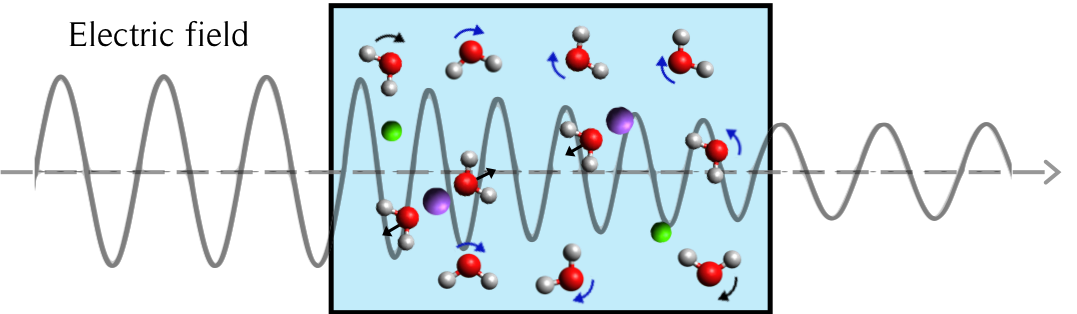
\includegraphics[width=0.85\figwidth]{chapters/Chapter1_Introduction/Graphs/DRS_Concept1.png} %The local modes are calculated on the XXX level, and reproduced with permission from ref. XXX. 
	\caption{Schematic representation of dielectric relaxation spectroscopy. If an external electric field is applied, water molecules will reorient towards the direction of the electric field. However, in the presence of ions, the degrees of rotational freedom of some water molecules are reduced or even locked in local structures referred to as solvation shells.}
	\label{DRSSchematic}
\end{figure}



Going one step further, we aim to determine hydration numbers by investigating the kinetic contribution to the depolarization experimental manner. In \textbf{Chapter~2}, we introduce the theoretical background and experimental methodology for the study of ion solvation using VNA-based DRS. In \textbf{Chapter~4}, we present a new method to extract hydration numbers based on the isotope dependence of the dielectric response. In this chapter, we aim to quantify the reduced cooperativity of water due to the local disruption  of the hydrogen-bond network. In \textbf{Chapter~5}, we apply this method to establish hydration numbers of a series of alkali-metal ions, and observe the ion-size dependence. Subsequently, in \textbf{Chapter~6}, we present similar analyses to estimate the number of water molecules affected by aqueous \ce{H+} and \ce{OH-} ions.



\subsection{Microscopic observation of solvating water molecules}



Femtosecond laser pulses have been used to perform ultrafast time-resolved vibrational spectroscopy (TRVS). This technique has been used to study molecular properties, e.g.\ molecular reorientation,\!\cite{Loparo2004,Rezus2005,Rezus2006,Thogersen2008,Shattuck2016} binding interactions,\!\cite{Eaves2005,Fecko2005,Baiz2015,Stevenson2015,Zhang2016} and energy equilibration.\!\cite{Woutersen1999,Piatkowski2009,Timmer2010} In this experimental approach, the way that light couples to the vibrational motion of molecules permits the exploration of structures down to the scale of a chemical bond ($\sim$1~\AA). An aspect of particular interest is that the vibrational resonances of molecules, as well as the associated vibrational relaxation rates, are sensitive to the structure and dynamics of the surrounding environment. This structure-dependent character allows us to assess the structural dynamics of solvating water molecules, as well as the properties of the hydrogen-bond network.



In particular, the vibrational properties of the hydroxyl groups of water molecules are affected by the hydrogen bonds that they donate, and consequently, by the strength of the hydrogen-bonding interactions in their vicinity.\!\cite{Lawrence2003,Auer2009,Bakker2010} A clear proof of this effect is observed in the OH-stretch resonance that shifts from 3657~cm$^{-1}$ in the gas phase (no hydrogen bonds) to lower frequencies around 3400~cm$^{-1}$ in the hydrogen-bonded liquid. This means that hydrogen bonds weaken the strength of the OH covalent bonds of water.



In electrolyte solutions, the vibrational dynamics of water molecules near ions further changes due to the strong local electric fields and the disruption of the hydrogen-bond network of water. In aqueous perchlorate (ClO$_4^{-}$) solutions, for example, there are two well-defined OH stretch bands: the first band associated with the bulk OH stretch vibration with a resonant frequency of 3400~cm$^{-1}$ and the second band at higher frequencies associated with OH oscillators that form weak hydrogen bonds with perchlorate ions.\!\cite{Timmer2010} One can thus selectively target and study the vibrational dynamics of solvating or bulk-like water molecules. As has been shown previously, TRVS experiments based on the OH stretch vibration are quite insensitive to the presence of cations.\!\cite{Omta2003,Omta2003a} This can be explained by the fact that no hydrogen bonds are donated to positive ions. This characteristic contrasts with DRS experiments.



\begin{figure}[t!]
	\centering
	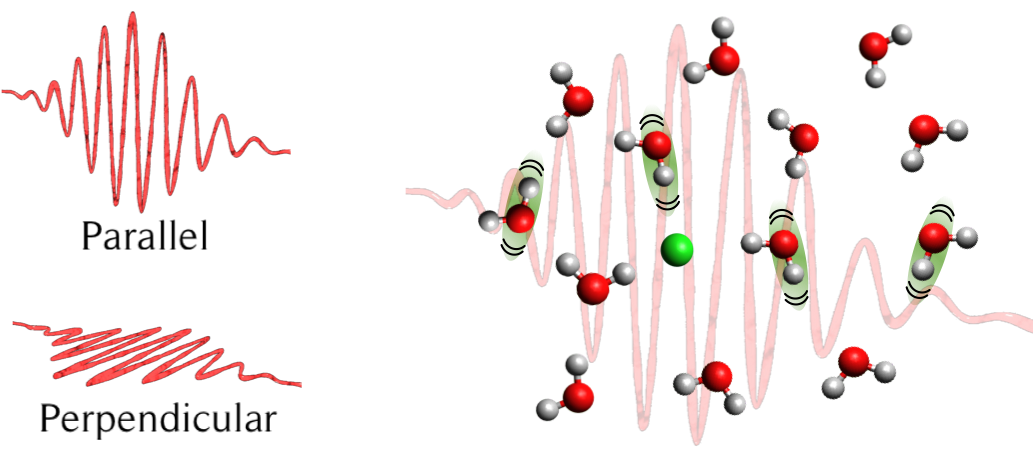
\includegraphics[width=0.85\figwidth]{chapters/Chapter1_Introduction/Graphs/TRVS_Concept1.png} %The local modes are calculated on the XXX level, and reproduced with permission from ref. XXX. 
	\caption{Schematic representation of time-resolved vibrational spectroscopy. An initial femtosecond pump pulse couples to local vibrational resonances of water molecules, which are afterwards tracked with a second femtosecond pulse called probe. In polarization-resolved TRVS, the sample is probed both in parallel and perpendicular configuration in order to observe molecular reorientation dynamics.}
	\label{TRVSSchematic}
\end{figure}


Polarization-resolved TRVS experiments provide direct information on the reorientation dynamics of the probed OH vibrations. Previous studies have shown a significant slowing down of the molecular dynamics upon the addition of ions. In fact, the reorientation dynamics of water in anionic solvation shells are strongly constrained to rotations within a cone around the axis defined by the directional hydrogen bond of the OH group to the anion.\!\cite{vanderPost2012,vanderPost2012a,vanderPost2013} In addition, the wiggling motion of the OH group bonded to the anion restricts the formation of hydrogen bonds between water molecules in the first solvation shell and the outer environment. Hence, the slow-down effect is limited to the first solvation shell, and the hydrogen-bond network is accordingly disrupted.\!\cite{Marcus2009} In contrast, aqueous sugar solutions have shown a slowing down effect that extends beyond the first solvation shell. This is explained by the fact that, instead of a disruptive effect, the hydroxyl groups of the sugar molecules form part of the hydrogen-bond network.\!\cite{Groot2014,Groot2015}


Protons (\ce{H+}) and hydroxide ions (\ce{OH-}) have the ability to form hydration complexes in which the excess charge is delocalized, and structural rearrangements lead to proton transfer between neighboring water molecules. This effect has been a fascinating subject of intense research in the last two decades. However, while a fairly large number of experimental efforts have been carried out on acid solutions,\!\cite{Woutersen2006,Moilanen2008,Peighambardoust2010,Liu2015,Fournier2018} only a few experimental studies in alkaline solutions have been reported.\!\cite{Roberts2009,Roberts2011,Mandal2014,Mandal2015,Biswas2017} As has been discussed before,\!\cite{Marx2010} this disparity can be explained from the classical view that hydroxide ions (\ce{OH-}, proton hole) mirror the effect of proton transfer via hydronium ions (\ce{H3O+}, proton excess). Nonetheless, recent theoretical studies have shown that \ce{OH-} and \ce{H3O+} ions have different structural properties, calling for the study of hydroxide ions as a subject of independent experimental research.\!\cite{Tuckerman2002,Chen2002,Sun2009,Bucher2010,Hassanali2011,Roberts2014,Chen2018a}


In \textbf{Chapter~3}, we introduce the theoretical background and experimental methodology for the study of intermolecular interactions in aqueous solutions using TRVS. \textbf{Chapters~7} and \textbf{8} focus on the study of structural properties in aqueous alkaline solutions using TRVS. In \textbf{Chapter~7}, we performed polarization-resolved measurements to explore whether hydroxide ions have an influence on the dynamics of water molecules beyond the first solvation shell. In \textbf{Chapter~8}, we explore whether the hydration complexes that hydroxide ions form can play a role in dissipating vibrational energy of surrounding molecules, an effect that has been observed in acidic solutions and has been attributed to the hydronium ion.\!\cite{Timmer2010} Finally, in \textbf{Chapter~9}, we study the solvation properties of aqueous phenolate ions using polarization-resolved TRVS and molecular dynamics simulations. 








